% Options for packages loaded elsewhere
\PassOptionsToPackage{unicode}{hyperref}
\PassOptionsToPackage{hyphens}{url}
%
\documentclass[
]{article}
\title{INFLATION, QUO VADIS?}
\author{Simon Wey}
\date{05 Juni 2022}

\usepackage{amsmath,amssymb}
\usepackage{lmodern}
\usepackage{iftex}
\ifPDFTeX
  \usepackage[T1]{fontenc}
  \usepackage[utf8]{inputenc}
  \usepackage{textcomp} % provide euro and other symbols
\else % if luatex or xetex
  \usepackage{unicode-math}
  \defaultfontfeatures{Scale=MatchLowercase}
  \defaultfontfeatures[\rmfamily]{Ligatures=TeX,Scale=1}
\fi
% Use upquote if available, for straight quotes in verbatim environments
\IfFileExists{upquote.sty}{\usepackage{upquote}}{}
\IfFileExists{microtype.sty}{% use microtype if available
  \usepackage[]{microtype}
  \UseMicrotypeSet[protrusion]{basicmath} % disable protrusion for tt fonts
}{}
\makeatletter
\@ifundefined{KOMAClassName}{% if non-KOMA class
  \IfFileExists{parskip.sty}{%
    \usepackage{parskip}
  }{% else
    \setlength{\parindent}{0pt}
    \setlength{\parskip}{6pt plus 2pt minus 1pt}}
}{% if KOMA class
  \KOMAoptions{parskip=half}}
\makeatother
\usepackage{xcolor}
\IfFileExists{xurl.sty}{\usepackage{xurl}}{} % add URL line breaks if available
\IfFileExists{bookmark.sty}{\usepackage{bookmark}}{\usepackage{hyperref}}
\hypersetup{
  pdftitle={INFLATION, QUO VADIS?},
  pdfauthor={Simon Wey},
  hidelinks,
  pdfcreator={LaTeX via pandoc}}
\urlstyle{same} % disable monospaced font for URLs
\usepackage{color}
\usepackage{fancyvrb}
\newcommand{\VerbBar}{|}
\newcommand{\VERB}{\Verb[commandchars=\\\{\}]}
\DefineVerbatimEnvironment{Highlighting}{Verbatim}{commandchars=\\\{\}}
% Add ',fontsize=\small' for more characters per line
\usepackage{framed}
\definecolor{shadecolor}{RGB}{248,248,248}
\newenvironment{Shaded}{\begin{snugshade}}{\end{snugshade}}
\newcommand{\AlertTok}[1]{\textcolor[rgb]{0.94,0.16,0.16}{#1}}
\newcommand{\AnnotationTok}[1]{\textcolor[rgb]{0.56,0.35,0.01}{\textbf{\textit{#1}}}}
\newcommand{\AttributeTok}[1]{\textcolor[rgb]{0.77,0.63,0.00}{#1}}
\newcommand{\BaseNTok}[1]{\textcolor[rgb]{0.00,0.00,0.81}{#1}}
\newcommand{\BuiltInTok}[1]{#1}
\newcommand{\CharTok}[1]{\textcolor[rgb]{0.31,0.60,0.02}{#1}}
\newcommand{\CommentTok}[1]{\textcolor[rgb]{0.56,0.35,0.01}{\textit{#1}}}
\newcommand{\CommentVarTok}[1]{\textcolor[rgb]{0.56,0.35,0.01}{\textbf{\textit{#1}}}}
\newcommand{\ConstantTok}[1]{\textcolor[rgb]{0.00,0.00,0.00}{#1}}
\newcommand{\ControlFlowTok}[1]{\textcolor[rgb]{0.13,0.29,0.53}{\textbf{#1}}}
\newcommand{\DataTypeTok}[1]{\textcolor[rgb]{0.13,0.29,0.53}{#1}}
\newcommand{\DecValTok}[1]{\textcolor[rgb]{0.00,0.00,0.81}{#1}}
\newcommand{\DocumentationTok}[1]{\textcolor[rgb]{0.56,0.35,0.01}{\textbf{\textit{#1}}}}
\newcommand{\ErrorTok}[1]{\textcolor[rgb]{0.64,0.00,0.00}{\textbf{#1}}}
\newcommand{\ExtensionTok}[1]{#1}
\newcommand{\FloatTok}[1]{\textcolor[rgb]{0.00,0.00,0.81}{#1}}
\newcommand{\FunctionTok}[1]{\textcolor[rgb]{0.00,0.00,0.00}{#1}}
\newcommand{\ImportTok}[1]{#1}
\newcommand{\InformationTok}[1]{\textcolor[rgb]{0.56,0.35,0.01}{\textbf{\textit{#1}}}}
\newcommand{\KeywordTok}[1]{\textcolor[rgb]{0.13,0.29,0.53}{\textbf{#1}}}
\newcommand{\NormalTok}[1]{#1}
\newcommand{\OperatorTok}[1]{\textcolor[rgb]{0.81,0.36,0.00}{\textbf{#1}}}
\newcommand{\OtherTok}[1]{\textcolor[rgb]{0.56,0.35,0.01}{#1}}
\newcommand{\PreprocessorTok}[1]{\textcolor[rgb]{0.56,0.35,0.01}{\textit{#1}}}
\newcommand{\RegionMarkerTok}[1]{#1}
\newcommand{\SpecialCharTok}[1]{\textcolor[rgb]{0.00,0.00,0.00}{#1}}
\newcommand{\SpecialStringTok}[1]{\textcolor[rgb]{0.31,0.60,0.02}{#1}}
\newcommand{\StringTok}[1]{\textcolor[rgb]{0.31,0.60,0.02}{#1}}
\newcommand{\VariableTok}[1]{\textcolor[rgb]{0.00,0.00,0.00}{#1}}
\newcommand{\VerbatimStringTok}[1]{\textcolor[rgb]{0.31,0.60,0.02}{#1}}
\newcommand{\WarningTok}[1]{\textcolor[rgb]{0.56,0.35,0.01}{\textbf{\textit{#1}}}}
\setlength{\emergencystretch}{3em} % prevent overfull lines
\providecommand{\tightlist}{%
  \setlength{\itemsep}{0pt}\setlength{\parskip}{0pt}}
\setcounter{secnumdepth}{-\maxdimen} % remove section numbering
\newlength{\cslhangindent}
\setlength{\cslhangindent}{1.5em}
\newlength{\csllabelwidth}
\setlength{\csllabelwidth}{3em}
\newlength{\cslentryspacingunit} % times entry-spacing
\setlength{\cslentryspacingunit}{\parskip}
\newenvironment{CSLReferences}[2] % #1 hanging-ident, #2 entry spacing
 {% don't indent paragraphs
  \setlength{\parindent}{0pt}
  % turn on hanging indent if param 1 is 1
  \ifodd #1
  \let\oldpar\par
  \def\par{\hangindent=\cslhangindent\oldpar}
  \fi
  % set entry spacing
  \setlength{\parskip}{#2\cslentryspacingunit}
 }%
 {}
\usepackage{calc}
\newcommand{\CSLBlock}[1]{#1\hfill\break}
\newcommand{\CSLLeftMargin}[1]{\parbox[t]{\csllabelwidth}{#1}}
\newcommand{\CSLRightInline}[1]{\parbox[t]{\linewidth - \csllabelwidth}{#1}\break}
\newcommand{\CSLIndent}[1]{\hspace{\cslhangindent}#1}
\ifLuaTeX
  \usepackage{selnolig}  % disable illegal ligatures
\fi

\begin{document}
\maketitle
\begin{abstract}
Die steigenden Inflationsraten beschäftigen nicht nur Konsumentinnen und
Konsu-menten immer stärker, sondern auch die Politik, die sich überlegen
muss, ob und wie sie gegen den Kaufkraftverlust vorgehen will.Die
preistreibenden Entwicklungen als Folge des Ukrainekriegs wie auch der
Folgen der Corona-Pandemie überlagern die zugrundeliegende Teuerung
aufgrund der expansiven Geldpolitik der Notenbanken in den letzten
Jahren.Eine vergleichbare Situation in Vergangenheit war die «Great
depression»-Krise in den 70er-Jahren. - Trotz einigen Parallelen gibt es
auch gewichtige Unterschiede bei den Ur-sachen, so etwa, dass die
Inflation stärker anstieg und sie sich breiter über die Bran-chen hinweg
manifestierte als heute. Durch die starke Intervention der
Nationalbanken wurde zudem das Wirtschaftswachstum abgeschwächt, wodurch
ein «hard landing» eintrat und das Phänomen der Stagflation geboren
wurde.Eine Mehrheit der von NZZ und KOF befragten Ökonomen gehen von
einem temporären Anstieg der Inflation aus. Dafür sprechen gewichtige
Gründe, etwa die sich abzeichnen-den Interventionen der Notenbanken, das
Auslaufen der fiskalischen Zahlungen zur Überwindung der Corona-Pandemie
oder auch die Überwindung der Auswirkungen der gestiegenen
Rohstoffpreise und der Lieferengpässe. Auch haben die strukturellen
Rahmenbedingungen die Inflation in Vergangenheit auf tieferem Niveau als
heute stabi-lisiert. Haben diese weiterhin Bestand, so dürften sich auch
diese negativ auf die Höhe der Inflation auswirken. Des Weiteren spielen
auch erwartungen eine zent-rale Rolle, die wiederum stark von der
Glaubwürdigkeit der Notenbanken abhängen.
\end{abstract}

\renewcommand{\figurename}{Abbildung}

\begin{figure} \centering
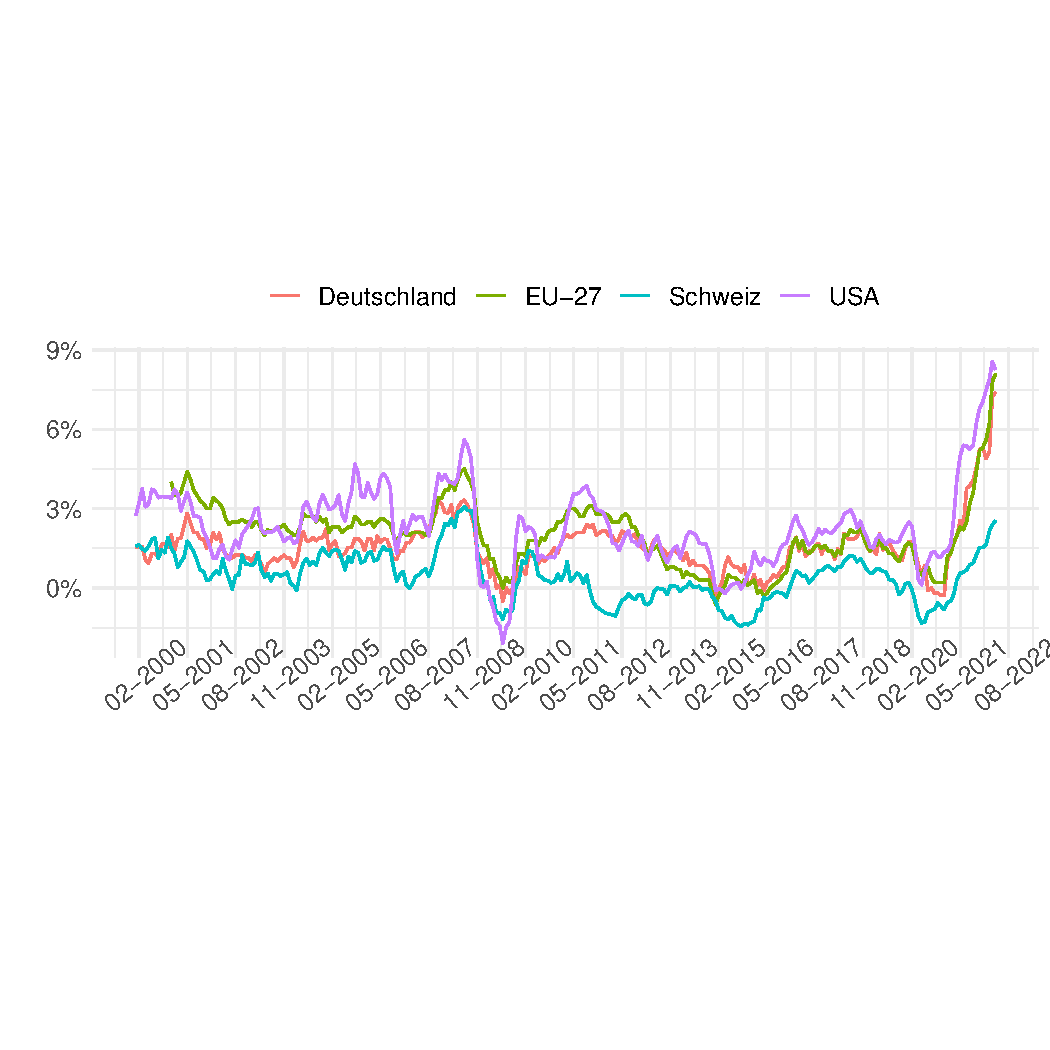
\includegraphics[trim={0 5.5cm 0 0cm },clip]{~/Repos/Inflation/graphics/infl_country_M.pdf}
\caption{Erwerbslosenquoten von Personen unterschiedlichen Alters in der Schweiz}
\label{Inf_M}
\end{figure}

\begin{figure} \centering
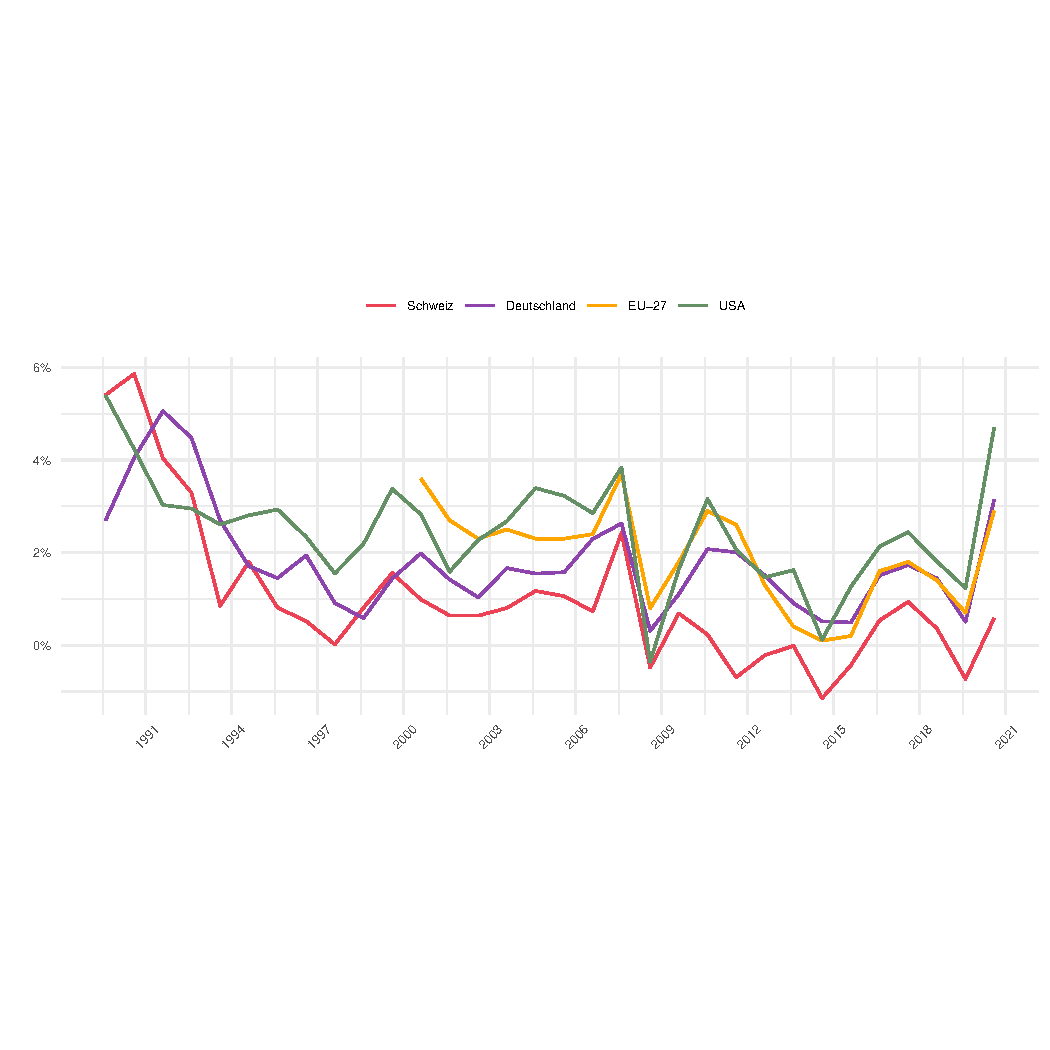
\includegraphics[trim={0 5.5cm 0 0cm },clip]{~/Repos/Inflation/graphics/infl_country_A.pdf}
\caption{Erwerbslosenquoten von Personen unterschiedlichen Alters in der Schweiz}
\label{Inf_A}
\end{figure}

\hypertarget{ausgangslage}{%
\section{Ausgangslage}\label{ausgangslage}}

Abberger K. und W. Nierhaus (2022) Zu hohe Teuerungsraten sind
ökonomisch schädlich und können zu sozialen und politischen
Verwer-fungen führen. Im März 2022 lagen raten in den USA bei 8.5
Prozent, in Deutschland bei 7.3 Prozent und in der EU-27 bei 7.8
Prozent. Dagegen war rate in der Schweiz mit 2.4 Prozent (vgl. Abbildung
\ref{Inf_M}) vergleichsweise moderat. Sie lag jedoch auch hierzulande
über dem oberen Rand des Zielbandes der Schweizerischen Nationalbank
(SNB). In Europa hatten die baltischen Staaten Litauen (16.6 Prozent),
Estland (14.8 Prozent) und Lettland (13.2 Prozent) sowie Tschechien
(11.9 Prozent) und die Niederlande (11.7 Prozent) neben der Türkei (61.1
Prozent) die höchsten Inflationsraten (vgl. Abbildung 4). Stark
getrieben ist der Anstieg von den Energie- und etwas weniger stark von
den Nahrungsmittelpreisen. Werden diese aus der Inflationsrate hinaus
gerechnet, so ist die Teuerung (Kerninflation) tiefer. In der Schweiz
lag sie im März bei 1.3 Pro-zent (vgl. Abbildung 2). Der politische
Druck steigt zunehmend, gegen den Kaufkraftverlust entschie-den
vorzugehen.

raten stiegen auch in Vergangenheit immer mal stark an, etwa während der
«Great de-pression» in den 70er-Jahren, wobei rate der Schweiz bis auf
wenige Ausnahmen meist tiefer verlief als denjenige der USA und der EU
(vgl. Abbildung 1). Auch war rate der Schweiz ab 2009 in mehreren Jahren
negativ, was die Reallöhne positiv beeinflusste und somit die Kaufkraft
stärkte.

Eine hohe Teuerung senkt die Kaufkraft und wirkt sich meist etwas
verzögert auch auf die Konsumen-tenstimmung aus. Dies zeigt sich auch
beim momentanen Anstieg, wobei sich zeigt, dass diese so-wohl in der
EU-27, in Deutschland, aber auch in der Schweiz seit etwa Sommer 2021
rückläufig ist und inzwischen in Deutschland bereits unter das Niveau
des Abfalls zu Beginn der Corona-Pandemie ge-fallen ist (vgl. Abbildung
5).

\begin{figure} \centering
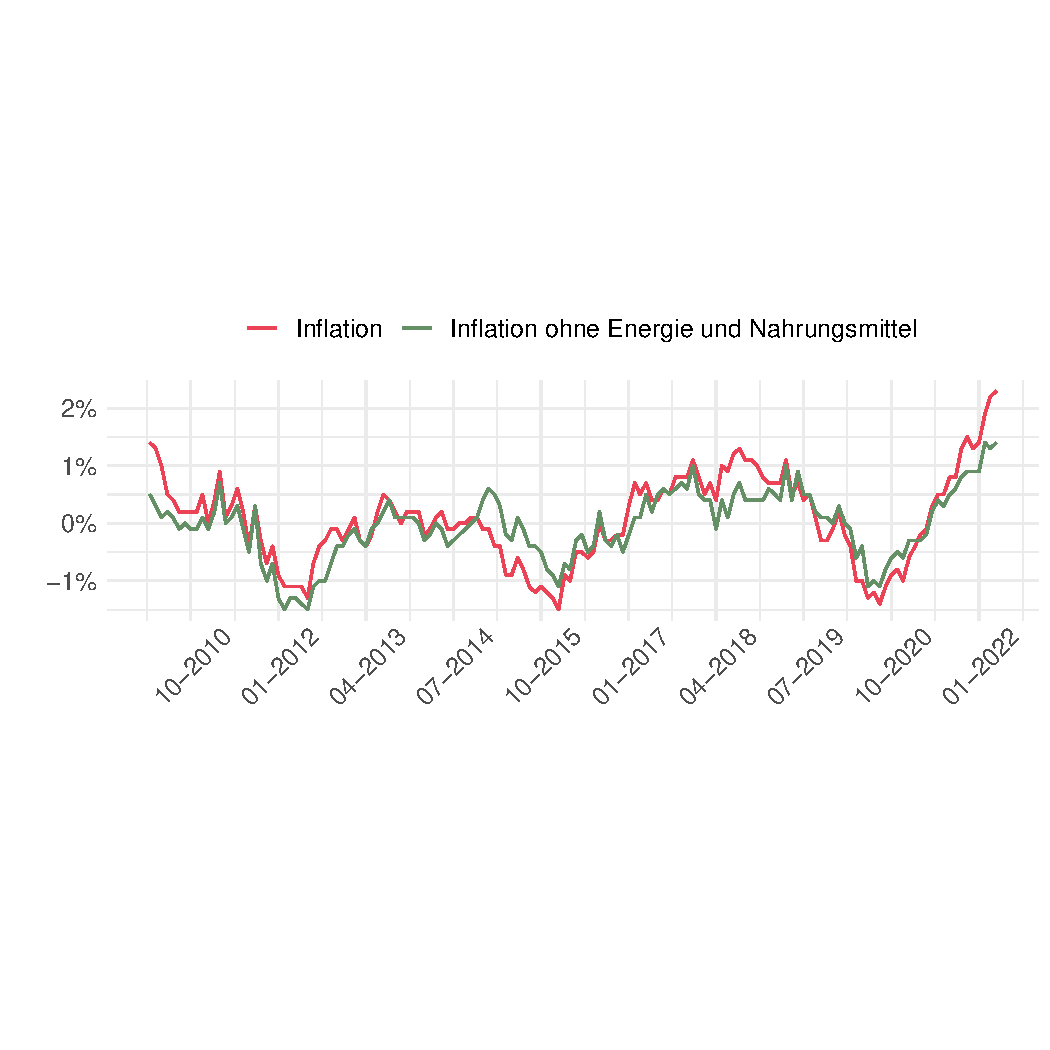
\includegraphics[trim={0 5.5cm 0 0cm},clip]{~/Repos/Inflation/graphics/infl_core_M.pdf}
\caption{Erwerbslosenquoten von Personen unterschiedlichen Alters in der Schweiz}
\label{Inf_A}
\end{figure}

\begin{figure} \centering
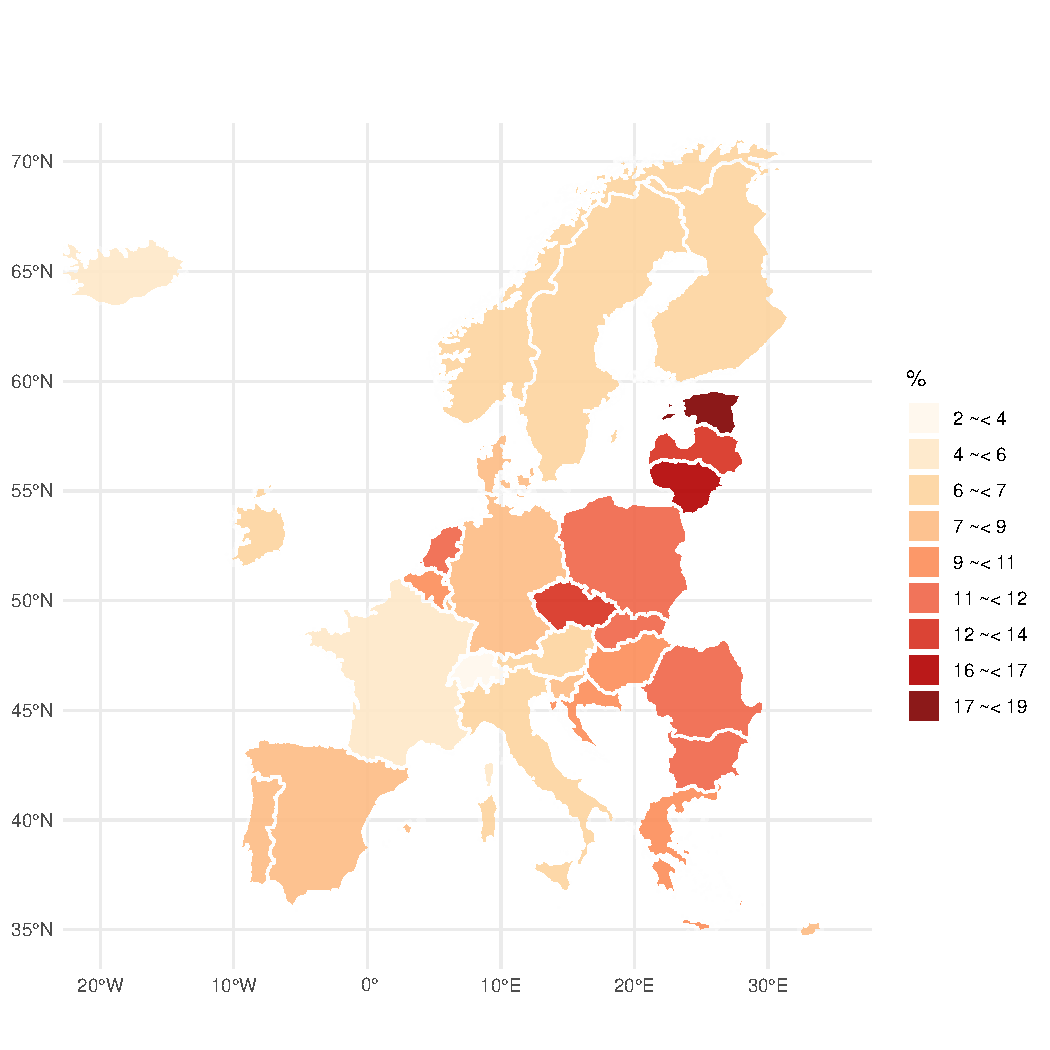
\includegraphics[trim={0 0cm 0 0cm},clip]{~/Repos/Inflation/graphics/MAP_Inflation_EU_202204.pdf}
\caption{Inflationsraten in Europa}
\label{Inf_A}
\end{figure}

\begin{figure} \centering
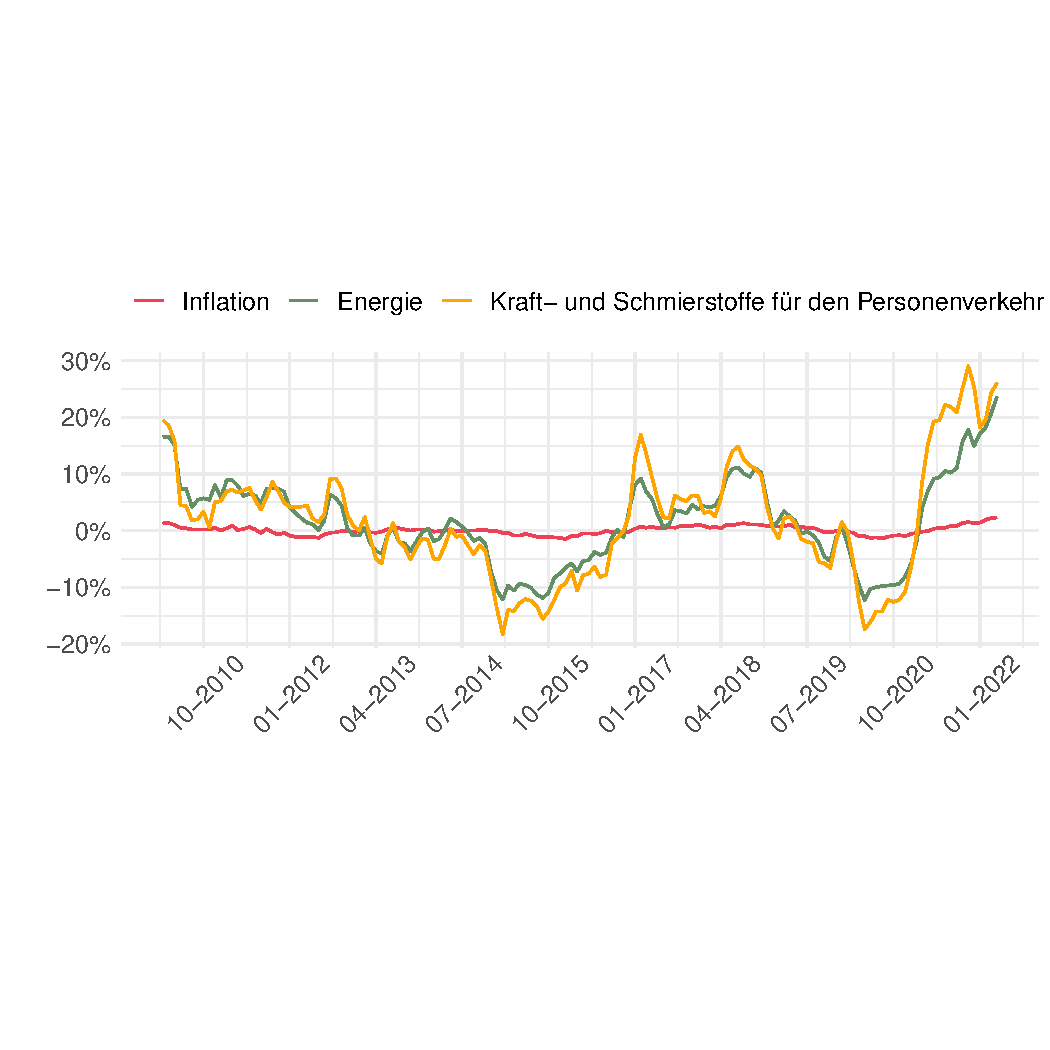
\includegraphics[trim={0 5.5cm 0 0cm },clip]{~/Repos/Inflation/graphics/infl_nrg_M.pdf}
\caption{Erwerbslosenquoten von Personen unterschiedlichen Alters in der Schweiz}
\label{Inf_A}
\end{figure}

\url{http://rmarkdown.rstudio.com}.

When you click the \textbf{Knit} button a document will be generated
that includes both content as well as the output of any embedded R code
chunks within the document. You can embed an R code chunk like this:

\begin{Shaded}
\begin{Highlighting}[]
\FunctionTok{summary}\NormalTok{(cars)}
\end{Highlighting}
\end{Shaded}

\begin{verbatim}
##      speed           dist       
##  Min.   : 4.0   Min.   :  2.00  
##  1st Qu.:12.0   1st Qu.: 26.00  
##  Median :15.0   Median : 36.00  
##  Mean   :15.4   Mean   : 42.98  
##  3rd Qu.:19.0   3rd Qu.: 56.00  
##  Max.   :25.0   Max.   :120.00
\end{verbatim}

\hypertarget{including-plots}{%
\subsection{Including Plots}\label{including-plots}}

You can also embed plots, for example:

\begin{figure} \centering
 \includegraphics[trim={0 50cm 0 0cm },clip]{~/Repos/Inflation/graphics/Cons_nood.pdf}
\caption{Erwerbslosenquoten von Personen unterschiedlichen Alters in der Schweiz}
\label{Inf_A}
\end{figure}

Note that the \texttt{echo\ =\ FALSE} parameter was added to the code
chunk to prevent printing of the R code that generated the plot.

\hypertarget{literatur}{%
\section*{Literatur}\label{literatur}}
\addcontentsline{toc}{section}{Literatur}

\hypertarget{refs}{}
\begin{CSLReferences}{1}{0}
\leavevmode\vadjust pre{\hypertarget{ref-kof}{}}%
Abberger K. und W. Nierhaus, 2022. Deutschland entgeht einer rezession?
Ökonomenstimme.

\end{CSLReferences}

\end{document}
